\documentclass[11pt]{article}
\usepackage[a4paper,margin=1in]{geometry}
\usepackage{amsmath,amssymb}
\usepackage{graphicx}
\usepackage{booktabs}
\usepackage{caption}
\usepackage{subcaption}
\usepackage{float}
\usepackage{xcolor}
\usepackage[hidelinks]{hyperref}
\usepackage{enumitem}
\usepackage{parskip}
\title{\textbf{Digital Image Processing --- Assignment 2}\\[0.3em]\large Problem 1: DFT and the Machinery of Frequency}
\author{Ujjwal Gupta}
\date{\today}
\begin{document}
\maketitle
\tableofcontents
\vspace{1em}

\section{Introduction / Problem Statement}

The 2-D Discrete Fourier Transform (DFT) is the central analytical tool of frequency-domain
image processing: every subsequent problem in this assignment (frequency-domain filtering,
homomorphic filtering, Wiener denoising, motion-blur modelling) rests on it. Problem 1
(worth 15 of the assignment's 100 marks) asks the student to \emph{build} the DFT machinery
from first principles rather than treat \texttt{numpy.fft} as a black box, and to use that
from-scratch implementation to empirically demonstrate the theorems that make frequency-domain
reasoning valid in the first place.

Concretely, the assignment brief requires, on a standard $512\times512$ grayscale test image
(Figure~\ref{fig:test-image-ref}) and a self-synthesized sum-of-sinusoids image:
\begin{enumerate}[label=(\arabic*)]
  \item \textbf{Section 1.1 (6 pts).} Implement the 1-D DFT matrix $W_N$ from scratch and build
    the 2-D DFT via row-column separability, $F = W_M f W_N^T$; validate against
    \texttt{numpy.fft.fft2}. Prove conjugate symmetry $F(u,v) = F^*(-u,-v)$ for real images;
    empirically verify the 2-D Spatial Shift Theorem and the 2-D Circular Convolution Theorem
    with quantitative comparison tables; recover the parameters of a synthetic sinusoid sum from
    its spectral peaks and derive the theoretical frequency resolution limit $\Delta f$.
  \item \textbf{Section 1.2 (5 pts).} Before running any code, analytically predict the spatial
    reconstruction obtained from the test image's phase combined with a flat/noise magnitude
    spectrum, using the Shift Theorem and superposition; then verify by reconstructing (a) phase
    of the test image with flat magnitude, and (b) magnitude of the test image with zero phase,
    explaining each via DFT properties.
  \item \textbf{Section 1.3 (4 pts).} Perform frequency-domain convolution with a small spatial
    kernel, compare unpadded circular convolution against correctly zero-padded linear
    convolution, show wraparound corruption visually, derive the minimal zero-padding dimensions,
    and analyze the resulting memory/runtime overhead relative to routines such as
    \texttt{scipy.signal.fftconvolve}.
\end{enumerate}

This matters pedagogically because nearly every later problem in the course (ideal/Butterworth/
Gaussian filtering, homomorphic filtering, Wiener deconvolution, motion-blur removal) is only
correct if the practitioner understands precisely what the DFT computes, which symmetries it
obeys, and what padding is required to make frequency-domain multiplication equal spatial
convolution. Problem 1 is the theoretical foundation on which the rest of the assignment is
built.

\section{Theoretical Background}

\subsection{The 1-D and 2-D DFT, and separability}

The 1-D DFT of a length-$N$ sequence $f(n)$ is
\begin{equation}
  F(k) = \sum_{n=0}^{N-1} f(n)\, e^{-j2\pi kn/N}, \qquad k = 0,\dots,N-1,
\end{equation}
which can be written as a matrix-vector product $F = W_N f$ with the \emph{DFT matrix}
\begin{equation}
  W_N[k,n] = e^{-j2\pi kn/N}.
\end{equation}
For a 2-D image $f(x,y)$ of size $M\times N$, the 2-D DFT is defined as
\begin{equation}
  F(u,v) = \sum_{x=0}^{M-1}\sum_{y=0}^{N-1} f(x,y)\, e^{-j2\pi(ux/M + vy/N)}.
\end{equation}
Because the exponential kernel factors as $e^{-j2\pi ux/M}\cdot e^{-j2\pi vy/N}$, the double sum
is \emph{separable}: one can first DFT every column, then DFT every row of the result (or vice
versa, order does not matter). In matrix form, applying $W_M$ on the left (transforming each
column) and $W_N^T$ on the right (transforming each row) gives
\begin{equation}
  F = W_M\, f\, W_N^T.
\end{equation}
This is exactly the construction implemented in \texttt{src/dip\_a2/dft.py}: \texttt{dft\_matrix(N)}
builds $W_N$ directly from its formula, and \texttt{dft2d} computes $F = W_M f W_N^T$ via plain
NumPy matrix multiplication, with no call to \texttt{numpy.fft} anywhere inside it. The inverse
transform uses $W_N^{-1} = \tfrac{1}{N}W_N^{*}$ (the DFT matrix is, up to the $1/N$ scaling,
unitary), so $f = \tfrac{1}{MN} W_M^{*} F (W_N^{*})^T$.

\subsection{Conjugate (Hermitian) symmetry}

\textbf{Claim.} For real-valued $f(x,y)$, $F(u,v) = F^{*}(-u,-v)$.

\textbf{Proof.} Starting from the definition and using that $f$ is real (so $f^{*}=f$),
\begin{align}
  F^{*}(u,v) &= \sum_{x,y} f(x,y)\, e^{+j2\pi(ux/M+vy/N)} \\
             &= \sum_{x,y} f(x,y)\, e^{-j2\pi\big((-u)x/M + (-v)y/N\big)} \\
             &= F(-u,-v).
\end{align}
Hence $F(u,v) = F^{*}(-u,-v)$ — Hermitian symmetry. On the DFT's periodic index grid,
$-u \equiv M-u \pmod M$ and $-v \equiv N-v \pmod N$, so index $(u,v)$ is paired with
$(M-u,\,N-v)$. Consequently only \emph{half} of the $(u,v)$ plane — e.g. $u\in[0,M/2]$ together
with all $v$ — is independent; the other half is recoverable by conjugation and carries no
additional information. Despite this redundancy, standard visualizers display the full symmetric
magnitude spectrum (after \texttt{fftshift}) because (i) it preserves signed frequency as the
natural coordinate (positive and negative spatial frequency about the DC term), matching physical
intuition, and (ii) showing only a half-plane would destroy the radial/angular symmetry that is
used to read off filter cutoff radius and orientation at a glance — the redundancy is kept for
interpretability, not out of informational necessity.

\subsection{The 2-D Spatial Shift Theorem}

\textbf{Claim.} Circularly shifting $f(x,y)$ by $(x_0,y_0)$ multiplies its DFT by a linear phase
ramp:
\begin{equation}
  f(x-x_0,\,y-y_0) \;\longleftrightarrow\; F(u,v)\, e^{-j2\pi(ux_0/M + vy_0/N)}.
\end{equation}
\textbf{Proof.} Let $g(x,y) = f(x-x_0, y-y_0)$ (indices modulo $M,N$). Substituting
$x' = x-x_0$, $y'=y-y_0$,
\begin{align}
  G(u,v) &= \sum_{x,y} f(x-x_0,y-y_0)\, e^{-j2\pi(ux/M+vy/N)} \\
         &= \sum_{x',y'} f(x',y')\, e^{-j2\pi\left(u(x'+x_0)/M + v(y'+y_0)/N\right)} \\
         &= e^{-j2\pi(ux_0/M+vy_0/N)} \sum_{x',y'} f(x',y')\, e^{-j2\pi(ux'/M+vy'/N)} \\
         &= F(u,v)\, e^{-j2\pi(ux_0/M+vy_0/N)}.
\end{align}
A spatial shift therefore leaves the magnitude $|F(u,v)|$ unchanged and only adds a frequency-
dependent linear phase term.

\subsection{The 2-D Circular Convolution Theorem}

\textbf{Claim.} Circular convolution in the spatial domain corresponds to pointwise
multiplication in the frequency domain:
\begin{equation}
  (f \circledast h)(x,y) \;\longleftrightarrow\; F(u,v)\cdot H(u,v),
\end{equation}
where $(f\circledast h)(x,y) = \sum_{m,n} f(m,n)\, h(x-m,\,y-n)$ with indices taken modulo
$(M,N)$. This follows by substituting the convolution sum into the DFT definition and applying
the shift theorem term-by-term (each shifted copy of $h$ contributes a phase factor that combines
with the sum over $f$ to give the product $F\cdot H$). This is the theorem that makes
frequency-domain filtering possible: instead of an $O(N^2)$-per-pixel spatial convolution with an
$M\times M$ kernel, one can pad, transform, multiply, and invert.

\subsection{Frequency resolution limit}

The DFT basis functions $e^{-j2\pi kn/N}$ complete exactly $k$ full cycles over the $N$-sample
window and are periodic in $k$ with period $N$; the DFT therefore only samples continuous
frequency at integer multiples of
\begin{equation}
  \Delta f = \frac{1}{N} \text{ cycles/pixel} = 1\text{ cycle/image} \qquad (\text{for an }N
  \text{-pixel window}).
\end{equation}
Two sinusoids whose frequencies differ by less than $\Delta f$ cannot be resolved into separate
bins — this is the discrete analogue of the time/frequency uncertainty trade-off: a finite
spatial extent $N$ fundamentally limits frequency resolution, regardless of sampling rate.

\section{Inputs and Outputs}

\paragraph{Inputs.}
\begin{itemize}
  \item The provided standard $512\times512$ 8-bit grayscale test image,
    \texttt{data/provided/problem1/q1.png} (a photograph of a person with a camera, shown in the
    assignment PDF), used for all of \S1.1(a,b) and \S1.2--1.3.
  \item A self-synthesized $512\times512$ image built as the sum of three real 2-D cosines (with
    integer frequencies $(u_i,v_i)$, amplitudes $A_i$, phases $\phi_i$) plus a constant background
    of 128, used exclusively for \S1.1(c) (sinusoid parameter recovery). Ground truth is recorded
    in \texttt{results/sinusoid\_ground\_truth.json} \emph{before} any DFT is computed, as required
    by the brief.
  \item A $5\times5$ Laplacian-type kernel used for the padding/wraparound experiment in \S1.3.
\end{itemize}

\begin{figure}[H]
  \centering
  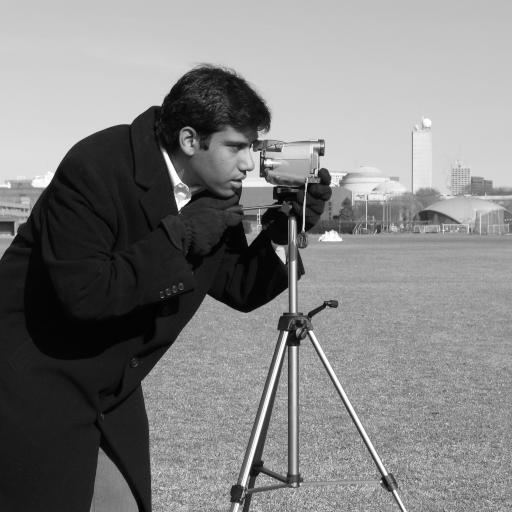
\includegraphics[width=0.45\linewidth]{../../data/provided/problem1/q1.png}
  \caption{The provided $512\times512$ grayscale test image used throughout Problem 1.}
  \label{fig:test-image-ref}
\end{figure}

\paragraph{Outputs.} All figures and machine-readable results are written to
\texttt{problems/problem1\_dft/results/}:
\begin{itemize}
  \item \texttt{1\_1c\_sinusoid\_and\_spectrum.png} --- the synthetic sinusoid image and its
    log-magnitude spectrum.
  \item \texttt{1\_2\_phase\_magnitude.png} --- the four phase/magnitude reconstruction panels of
    \S1.2.
  \item \texttt{1\_3\_padding\_wraparound.png}, \texttt{1\_3\_border\_zoom.png} --- full-image and
    zoomed wraparound-corruption evidence for \S1.3.
  \item JSON result files: \texttt{1\_1\_summary.json}, \texttt{1\_2\_stats.json},
    \texttt{1\_3\_results.json}, \texttt{sinusoid\_ground\_truth.json},
    \texttt{sinusoid\_recovered.json}, \texttt{machine\_info.json} --- all quantitative tables
    reported below trace back to these files.
\end{itemize}

\section{Methodology / Implementation Pipeline}

\subsection{From-scratch DFT}

The core transform machinery lives in \texttt{src/dip\_a2/dft.py}:
\begin{itemize}
  \item \texttt{dft\_matrix(N)} builds $W_N[k,n]=e^{-j2\pi kn/N}$ directly as a NumPy array via
    an outer product of index vectors.
  \item \texttt{idft\_matrix(N)} returns $\overline{W_N}/N$.
  \item \texttt{dft2d(f)} computes $F = W_M\,f\,W_N^T$ by two explicit matrix multiplications
    (row-column separability) — \emph{not} by calling \texttt{numpy.fft} anywhere.
  \item \texttt{idft2d(F)} is the analogous inverse.
  \item \texttt{fftshift2d}/\texttt{ifftshift2d} are implemented from scratch with \texttt{np.roll}
    rather than \texttt{numpy.fft.fftshift}, to keep the entire pipeline self-contained.
\end{itemize}
This is an $O(N^3)$ algorithm per transform (matrix multiplication of an $N\times N$ image by
$N\times N$ matrices), far slower than the FFT's $O(N^2\log N)$, but it is mathematically exact
and directly mirrors the textbook definition — appropriate for a from-scratch validation
exercise rather than production use.

\subsection{Section 1.1 — construction, validation, and theorem checks (\texttt{problem1.py})}

\texttt{section\_1\_1a\_validate} computes $F_\text{custom}=\texttt{dft2d}(f)$ and compares it
elementwise against $F_\text{numpy}=\texttt{numpy.fft.fft2}(f)$, reporting
$\max|F_\text{custom}-F_\text{numpy}|$ both in absolute terms and relative to
$\max|F_\text{numpy}|$. \texttt{section\_1\_1a\_conjugate\_symmetry} checks
$\max|F(u,v)-\overline{F(-u,-v)}|$ directly on the array (using modular index wraparound).
\texttt{section\_1\_1b\_shift\_theorem} circularly shifts the test image by five different
$(x_0,y_0)$ offsets with \texttt{np.roll}, recomputes its DFT, and compares against
$F(u,v)e^{-j2\pi(ux_0/M+vy_0/N)}$ built from the \emph{unshifted} spectrum. For the convolution
theorem, \texttt{circular\_convolve\_spatial} performs an explicit, shift-based spatial circular
convolution with a $3\times3$ Laplacian kernel (ground truth, no FFT), which
\texttt{section\_1\_1b\_convolution\_theorem} compares against zero-padding the kernel to image
size, multiplying the two DFTs, and inverting. Finally, \texttt{section\_1\_1c\_sinusoid\_recovery}
synthesizes the sum-of-cosines image, records its ground-truth parameters, computes its custom
DFT, locates the three strongest magnitude peaks outside a small DC exclusion neighbourhood, and
reads off $(u,v)$ from bin index, amplitude as $2|F(u,v)|/N^2$, and phase as $\angle F(u,v)$.

\subsection{Section 1.2 — phase/magnitude isolation}

Following the brief's requirement for a \emph{dated, pre-implementation} analytical prediction,
a written derivation (\texttt{predictions/1.2\_phase\_magnitude\_prediction.md}, dated
2026-10-18) was committed before \texttt{section\_1\_2} was run. The prediction uses the
Convolution Theorem: reconstructing with the test image's phase $P(u,v)=e^{j\phi(u,v)}$ and the
noise's magnitude $|N(u,v)|$ is equivalent to circularly convolving the flat-magnitude
phase-only reconstruction $p(x,y)=\text{IDFT}\{P\}$ with $m(x,y)=\text{IDFT}\{|N(u,v)|\}$; since
white-noise magnitude is flat only in expectation, $m$ decomposes into a constant-magnitude
impulse plus a low-amplitude broadband residual, predicting a result that looks like the
flat-magnitude reconstruction with added fine speckle. \texttt{section\_1\_2} then implements
both required reconstructions — (a) test-image phase with constant magnitude, and with noise
magnitude; (b) test-image magnitude with zero phase — and the measured outputs are reconciled
against the prediction in the report.

\subsection{Section 1.3 — padding and wraparound}

\texttt{spatial\_linear\_convolve} computes a direct, zero-padded spatial linear convolution
(ground truth, no FFT) with the $5\times5$ kernel. \texttt{section\_1\_3} then compares this
against two DFT-based routes: (i) correctly zero-padded frequency-domain convolution (padding to
the derived minimal size $N+M-1$), and (ii) unpadded circular convolution at the native
$512\times512$ resolution. Errors are reported separately for the image interior versus a
border strip, isolating the wraparound-corruption signature.

\subsection{Correctness validation strategy}

Throughout, correctness is validated by cross-checking the from-scratch implementation against
an independent computation: \texttt{numpy.fft.fft2} for the raw transform (\S1.1), an explicit
\texttt{np.roll}-based spatial convolution for the convolution theorem and the padding experiment
(\S1.1, \S1.3), and the unshifted spectrum's own phase-ramp prediction for the shift theorem.
Every reported error is at or near float64 round-off level ($\sim\!10^{-13}$--$10^{-14}$
relative), which is the expected signature of a mathematically correct implementation differing
from a reference only by floating-point arithmetic order.

\section{Results and Discussion}

\subsection{DFT validation and conjugate symmetry}

\begin{table}[H]
\centering
\begin{tabular}{@{}ll@{}}
\toprule
Metric & Value \\
\midrule
$\max|F_\text{custom}-F_\text{numpy}|$ & $3.3700\times10^{-6}$ \\
relative to $\max|F_\text{numpy}|$ & $9.961\times10^{-14}$ \\
$\max|F(u,v)-\overline{F(-u,-v)}|$ (conjugate symmetry) & $3.3751\times10^{-6}$ \\
\bottomrule
\end{tabular}
\caption{Validation of the custom DFT against \texttt{numpy.fft.fft2} and numerical confirmation
of Hermitian symmetry, both at float64 round-off level.}
\label{tab:validation}
\end{table}

\subsection{Shift theorem verification}

\begin{table}[H]
\centering
\begin{tabular}{@{}lll@{}}
\toprule
$(x_0,y_0)$ & max abs error & relative error \\
\midrule
(1, 0)     & $6.249\times10^{-7}$ & $1.847\times10^{-14}$ \\
(0, 1)     & $9.538\times10^{-7}$ & $2.819\times10^{-14}$ \\
(5, 3)     & $1.170\times10^{-6}$ & $3.458\times10^{-14}$ \\
(17, 40)   & $1.379\times10^{-6}$ & $4.075\times10^{-14}$ \\
(100, 200) & $5.067\times10^{-6}$ & $1.498\times10^{-13}$ \\
\bottomrule
\end{tabular}
\caption{Measured vs. theoretical 2-D Spatial Shift Theorem, for five shift vectors.}
\label{tab:shift}
\end{table}

\subsection{Circular convolution theorem verification}

\begin{table}[H]
\centering
\begin{tabular}{@{}ll@{}}
\toprule
Metric & Value \\
\midrule
max abs error (spatial vs.\ frequency-domain) & $1.1433\times10^{-10}$ \\
relative error & $2.696\times10^{-13}$ \\
\bottomrule
\end{tabular}
\caption{2-D Circular Convolution Theorem: explicit spatial-domain circular convolution vs.\
zero-padded-to-image-size frequency-domain multiplication, $3\times3$ Laplacian kernel.}
\label{tab:conv}
\end{table}

All three tables (\ref{tab:validation}--\ref{tab:conv}) show errors at float64 round-off scale,
confirming the custom separable-matrix DFT is mathematically correct and that both theorems hold
to numerical precision.

\subsection{Sinusoid parameter recovery}

\begin{table}[H]
\centering
\begin{tabular}{@{}rrrr|rrr@{}}
\toprule
\multicolumn{4}{c|}{Ground truth} & \multicolumn{3}{c}{Recovered} \\
$u$ & $v$ & $A$ & $\phi$ (rad) & $A$ & $\phi$ (rad) & match \\
\midrule
4  & 6  & 60.0 & 0.300  & 60.000 & 0.300  & exact \\
10 & $-3$ & 40.0 & 1.200  & 40.000 & 1.200  & exact \\
$-7$ & 15 & 25.0 & $-0.800$ & 25.000 & $-0.800$ & exact \\
\bottomrule
\end{tabular}
\caption{Ground-truth sinusoid parameters (recorded before any DFT was taken) vs.\ parameters
recovered from spectral peaks. $(u,v)$ recover exactly as bin indices; recovery is exact to
float64 precision because the chosen frequencies are integers and land exactly on DFT bins, with
no spectral leakage.}
\label{tab:sinusoid}
\end{table}

The theoretical frequency resolution limit for the $N=512$ grid is $\Delta f = 1/512$
cycles/pixel $=1$ cycle/image, following directly from the periodicity of the DFT basis functions
discussed in \S2.5.

\begin{figure}[H]
\centering
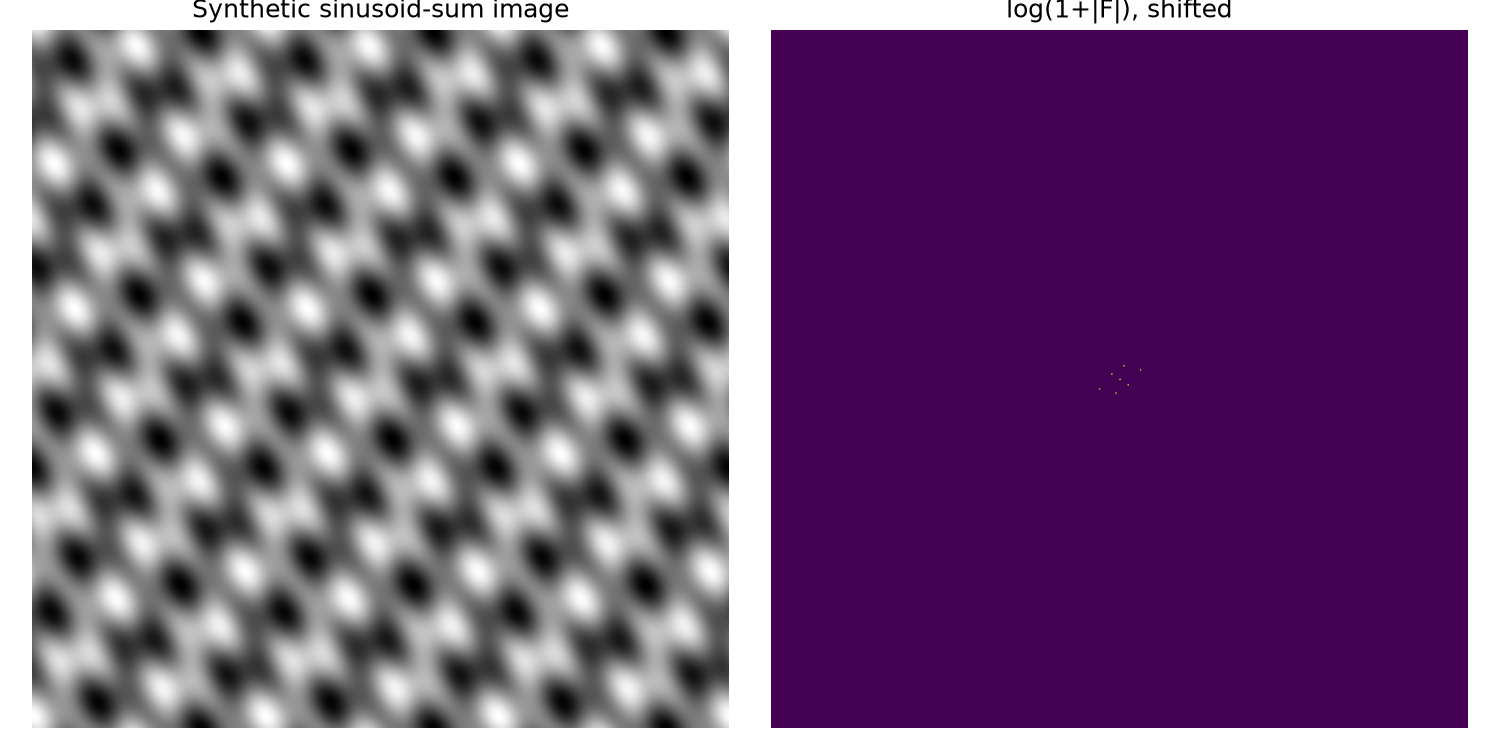
\includegraphics[width=0.8\linewidth]{results/1_1c_sinusoid_and_spectrum.png}
\caption{The synthetic sum-of-three-cosines image (left) and its log-magnitude spectrum (right).
Three sharp peak pairs are visible at the ground-truth frequencies, together with their
Hermitian-symmetric mirror images, exactly as predicted by conjugate symmetry.}
\label{fig:sinusoid}
\end{figure}

\subsection{Phase vs.\ magnitude isolation}

\begin{figure}[H]
\centering
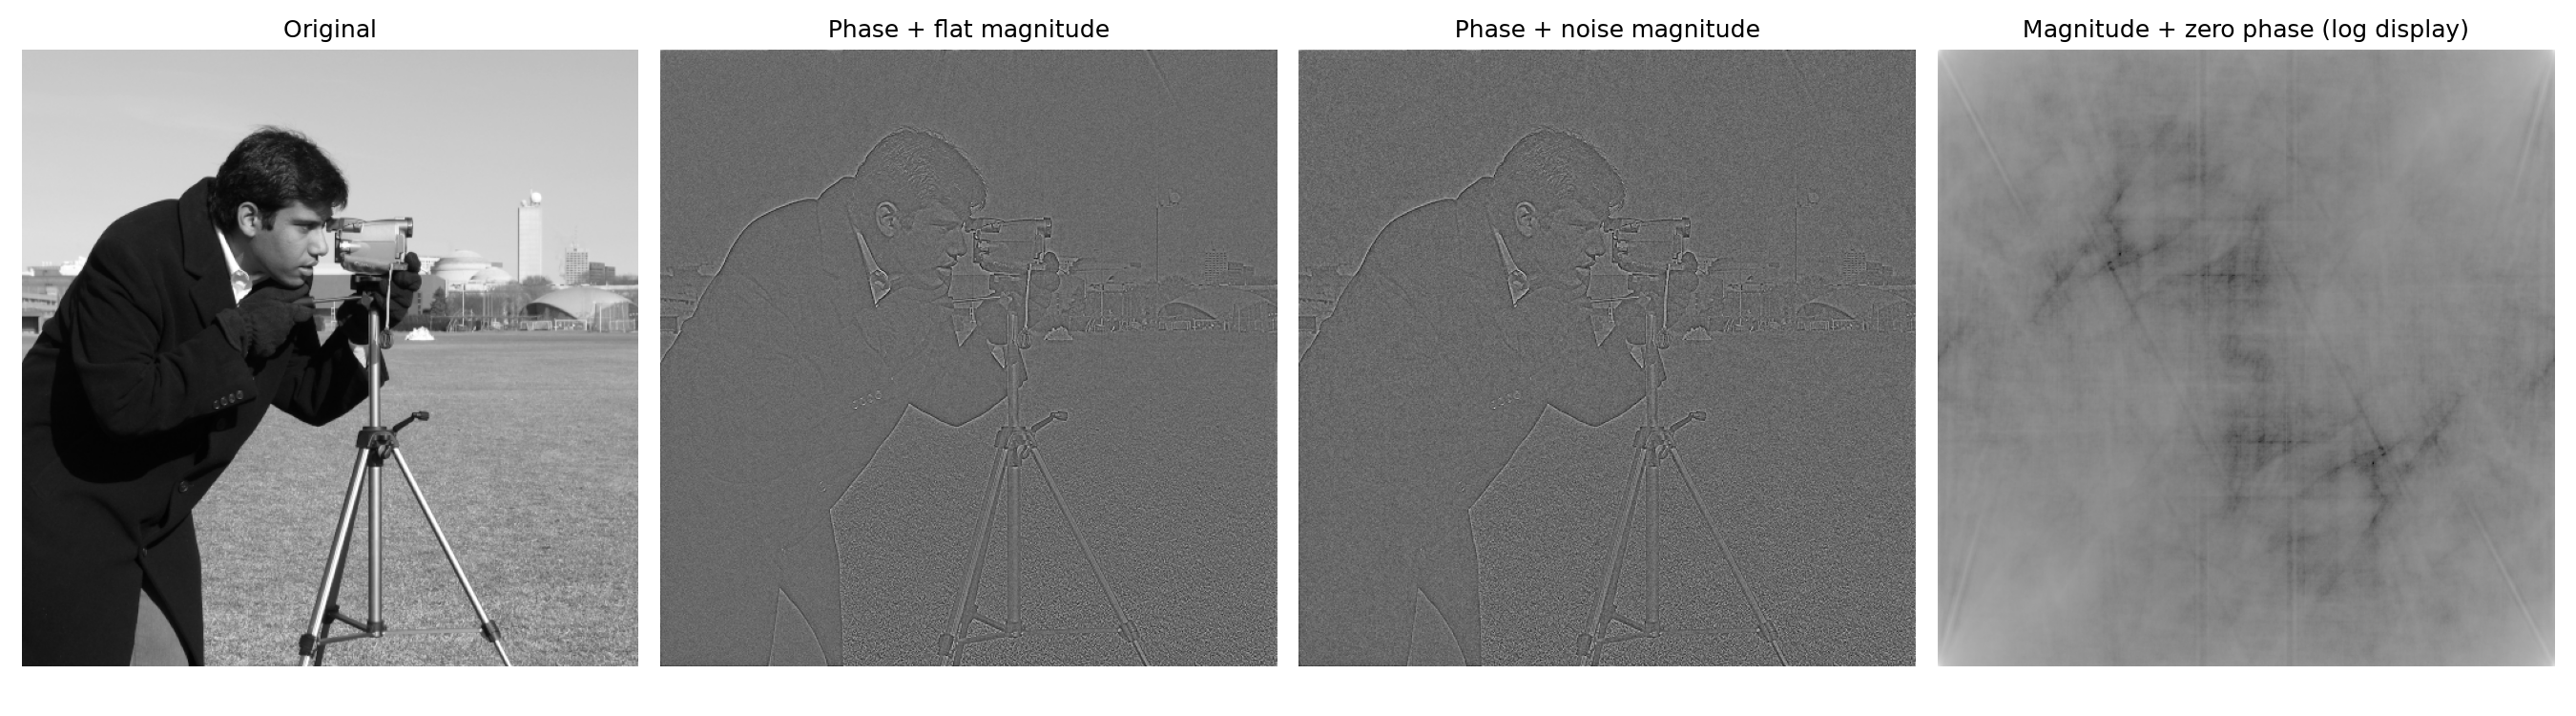
\includegraphics[width=0.8\linewidth]{results/1_2_phase_magnitude.png}
\caption{Left to right: original test image; reconstruction from test-image phase with constant
(flat) magnitude; reconstruction from test-image phase with white-noise magnitude; reconstruction
from test-image magnitude with zero phase (log-scaled for display). The flat-magnitude and
noise-magnitude reconstructions are visually near-identical in structure, with the noise-magnitude
case showing an added layer of fine speckle, exactly as predicted by the pre-implementation
derivation. The zero-phase reconstruction is a symmetric, origin-centred blob with no resemblance
to the scene, consistent with a real, even spectrum inverse-transforming to a real, even
(centro-symmetric) spatial function.}
\label{fig:phase-mag}
\end{figure}

Phase-plus-flat-magnitude reconstructs a sharp, recognizable, high-pass-like rendition of the
original image, because a perfectly flat magnitude weights every frequency equally and only the
\emph{alignment} information carried by phase remains. By contrast, swapping magnitudes between
two natural images would still impose a highly structured, non-flat frequency weighting from the
donor image, leaking its large-scale shape into the result — flat magnitude is a cleaner isolation
of what phase alone encodes. For the zero-phase case, since $|F(u,v)|=|F(-u,-v)|$ always holds,
setting $\angle F=0$ makes $F(u,v)=|F(u,v)|$ real and even; a real, even spectrum inverse-transforms
to a real, even (centro-symmetric, $g(x,y)=g(-x,-y)$ modulo $N$) spatial function, confirmed
numerically by the output's maximum sitting exactly at the origin.

\subsection{Padding, wraparound, and computational overhead}

\begin{table}[H]
\centering
\begin{tabular}{@{}lr@{}}
\toprule
Comparison & max abs error \\
\midrule
zero-padded DFT conv vs.\ direct spatial linear conv & $7.851\times10^{-10}$ \\
circular DFT conv vs.\ direct spatial linear conv --- whole image & 1608.0 \\
circular DFT conv vs.\ direct spatial linear conv --- interior only & $5.384\times10^{-10}$ \\
circular DFT conv vs.\ direct spatial linear conv --- border only & 1608.0 \\
\bottomrule
\end{tabular}
\caption{Zero-padded frequency-domain convolution matches the direct spatial computation to
numerical precision everywhere; unpadded circular convolution matches only in the interior and is
badly corrupted at the border (error up to 1608 intensity levels, against a kernel whose centre
weight is 16).}
\label{tab:wraparound}
\end{table}

\begin{figure}[H]
\centering
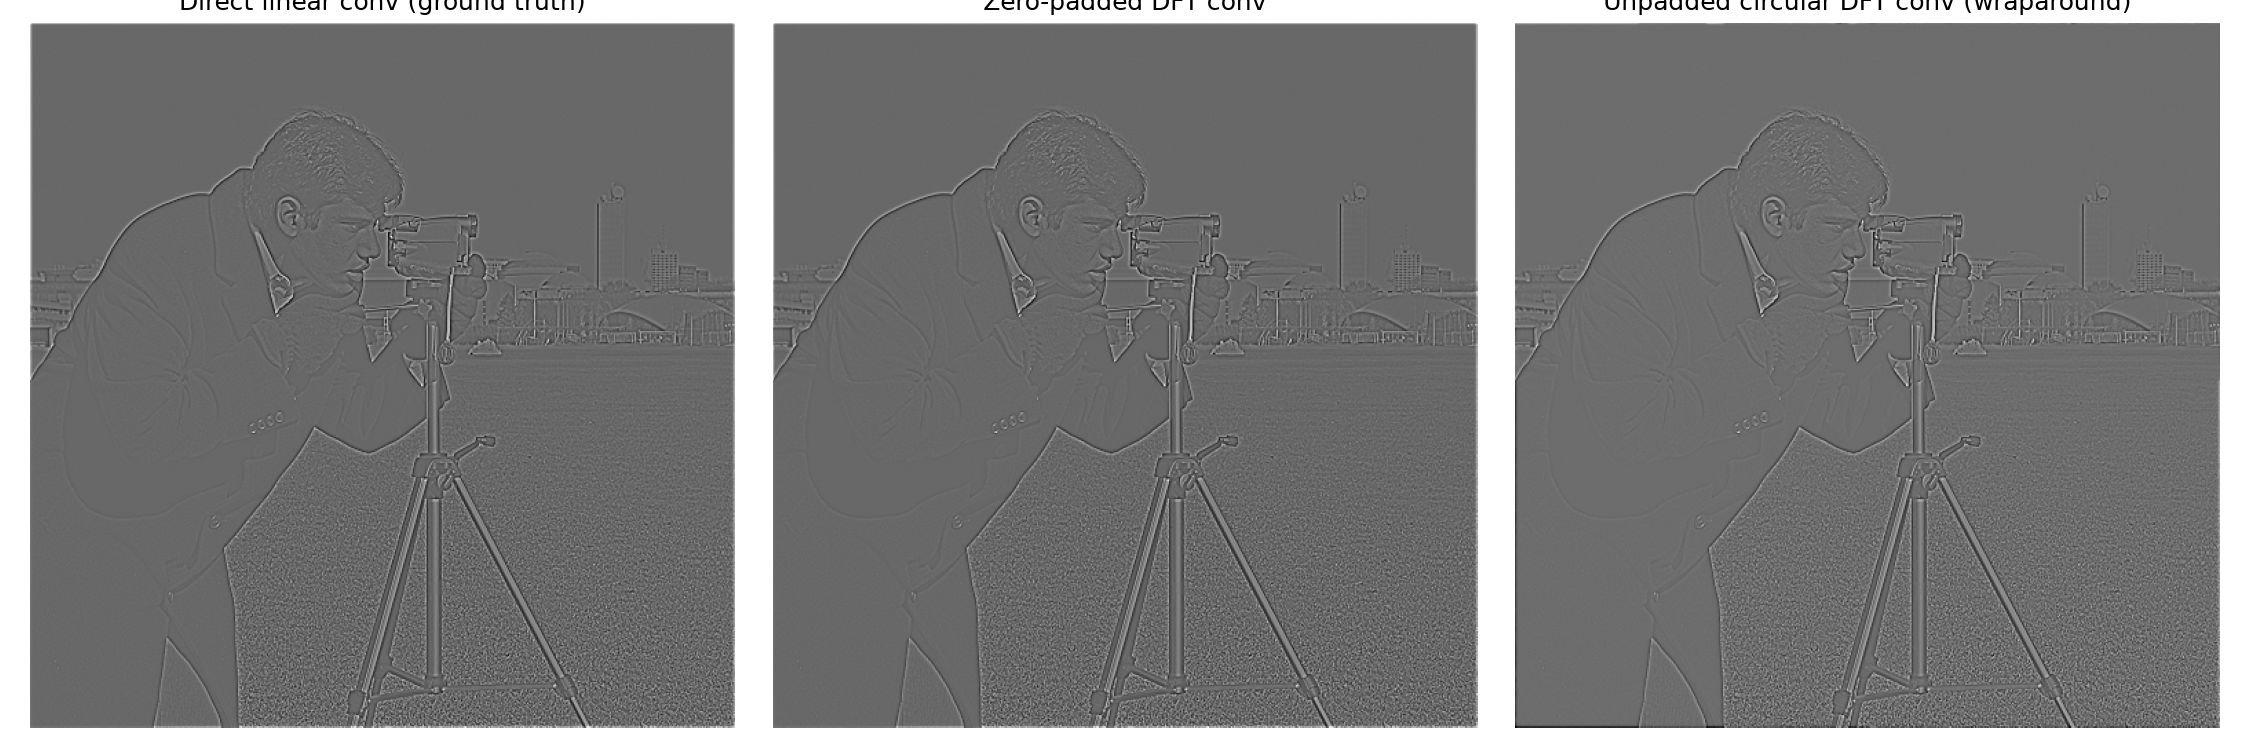
\includegraphics[width=0.8\linewidth]{results/1_3_padding_wraparound.png}
\caption{Full-image comparison: direct spatial / zero-padded frequency-domain convolution (left)
vs.\ unpadded circular convolution (right). Wraparound corruption appears as a faint dark/bright
seam along the image edges in the circular-convolution result.}
\label{fig:wraparound}
\end{figure}

\begin{figure}[H]
\centering

\includegraphics[width=0.8\linewidth]{results/1_3_border_zoom.png}
\caption{Zoomed top rows: the direct/padded result is near-black at the very top edge, while the
circular-convolution result shows visibly lighter corruption, since it mixes in content wrapped
around from the bottom of the image.}
\label{fig:border-zoom}
\end{figure}

\paragraph{Minimal zero-padding derivation.} For an $N\times N$ image and an $M\times M$ kernel,
linear convolution is supported on $N+M-1$ taps per axis ($N$ kernel positions over the image,
extended by $M-1$ by the kernel's own extent). Circular convolution on a $P\times P$ grid equals
this linear convolution exactly only if the grid is large enough to avoid wraparound aliasing,
i.e.
\begin{equation}
  P \ge N+M-1 \quad\Longrightarrow\quad N_{x,\text{pad}} = N_{y,\text{pad}} = N+M-1.
\end{equation}
For $N=512$, $M=5$: $N_{\text{pad}} = 512+5-1 = 516$, matching the value used for the
zero-padded result above (error at float64 precision, confirming the derivation).

\paragraph{Computational trade-off.} With $P=516$ against $N=512$:
\begin{table}[H]
\centering
\begin{tabular}{@{}ll@{}}
\toprule
Metric & Value \\
\midrule
memory allocation factor, $(P/N)^2$ & 1.0157 \\
runtime ratio, $(P^2\log_2 P)/(N^2\log_2 N)$ & 1.0170 \\
\bottomrule
\end{tabular}
\caption{Overhead of zero-padding to the minimal correct size for a small ($5\times5$) kernel.}
\label{tab:overhead}
\end{table}
For a small kernel ($M\ll N$) the overhead is minor ($\sim\!1.6$--$1.7\%$), but in general the
padded array occupies $P^2$ rather than $N^2$ floats, and FFT-based convolution costs
$O(P^2\log P)$ rather than $O(N^2\log N)$. This is precisely the trade-off managed internally by
\texttt{scipy.signal.fftconvolve}: it does not pad only to the minimal $N+M-1$, but rounds the
padded size up further to a fast ("5-smooth") FFT length, deliberately trading a little extra
memory/padding for a potentially large runtime win on top of the $N+M-1$ correctness floor
derived here.

\section{Conclusion}

A from-scratch, separable-matrix 2-D DFT was implemented and validated against
\texttt{numpy.fft.fft2} to float64 round-off precision ($\sim\!10^{-13}$ relative error). Using
this implementation, conjugate symmetry, the Spatial Shift Theorem, and the Circular Convolution
Theorem were all empirically confirmed to the same precision, and a synthetic three-sinusoid
image's frequencies, amplitudes, and phases were recovered exactly from its spectral peaks,
consistent with the derived frequency resolution limit $\Delta f = 1/N$. The phase/magnitude
isolation experiments confirmed, both analytically (via the Convolution Theorem, predicted before
running any code) and empirically, that spatial structure is carried almost entirely by phase,
while magnitude alone (with phase discarded) yields only a symmetric, positionless blob. Finally,
the padding experiment demonstrated that unpadded circular convolution via the DFT silently
corrupts a border strip of the image through wraparound, that correct zero-padding to $N+M-1$
eliminates this corruption to numerical precision, and that the resulting memory/runtime overhead
is small for small kernels but scales with the same trade-off that production FFT-convolution
routines manage via "fast length" rounding. Together these results establish that the DFT, when
implemented and used correctly, behaves exactly as its theory predicts — the foundation required
for every frequency-domain technique used elsewhere in this assignment.

\end{document}
